% !TeX root = RJwrapper.tex
\title{spinifex: An R Package for Creating a Manual Tour of Low-dimensional
Projections of Multivariate Data}
\author{by Nicholas Spyrison, Dianne Cook}

\maketitle

\abstract{%
Dynamic low-dimensional linear projections of multivariate data
collectively known as \textbf{tours} provide an important tool for
exploring multivariate data and models. The R package \pkg{tourr}
provides functions for several types of tours: grand, guided, little,
local and frozen. Each of these can be viewed dynamically, or saved into
a data object for animation. This paper describes a new package,
\pkg{spinifex}, to provide a manual tour, that allows the coefficient
for a single variable to be controlled. The variable is rotated fully
into the projection, or completely out of the projection. The resulting
sequence of projections can be displayed using animation, with functions
from either the \pkg{plotly} and \pkg{gganimate} packages. By varying
the coefficient of a single variable, it is possible to explore the
sensitivity of structure in the projection to that variable. It is
particularly useful when used with a projection pursuit guided tour to
simplify and understand the solution. The use of the manual tour for
studying the sensitivity of structure, in a projection, to specific
variable contributions, is illustrated using particle physics data.
}


\bibliography{spinifex_paper}

\hypertarget{introduction}{%
\section{Introduction}\label{introduction}}

Exploring multivariate spaces is a challenging task, increasingly so as
dimensionality increases. Traditionally, static low-dimensional
projections are used to display multivariate data in two dimensions,
such as principal component analysis, linear discriminant spaces or
projection pursuit. These are useful for finding relationships between
multiple variables, but they are limited because they show only a
glimpse of the high-dimensional space. An alternative approach is to use
a tour (Asimov \protect\hyperlink{ref-asimov_grand_1985}{1985}) of
dynamic linear projections, to look at many different low-dimensional
projections. Tours can be considered to extend the dimensionality of
visualization, which is important as data and models exist in more than
3D. The package \CRANpkg{tourr} (Wickham et al.
\protect\hyperlink{ref-wickham_tourr_2011}{2011}) provides a platform
for generating tours. It has many types of tours available, and many
types of displays possible. A user can make a grand, guided, little,
local or frozen tour, and display the resulting projected data as a
scatterplot, density plot, histogram, or even as Chernoff faces if the
projection dimension is more than 3.

This work adds a manual tour to the collection. The manual tour was
described in Cook and Buja
(\protect\hyperlink{ref-cook_manual_1997}{1997}) and allows a user to
control the projection coefficients of a selected variable in a 2D
projection. The manipulation of these coefficients allows the analyst to
explore their sensitivity to the structure within the projection. As
manual tours operate on only one variable at a time, they are
particularly useful once a feature of interest has been identified.

One way to identify ``interesting'' features is with the use of a guided
tour (Cook et al. \protect\hyperlink{ref-cook_grand_1995}{1995}). Guided
tours select a very specific path, which approaches a projection that
optimizes an objective-function. The optimization is conducted in a
manner similar to simulated annealing (Kirkpatrick, Gelatt, and Vecchi
\protect\hyperlink{ref-kirkpatrick_optimization_1983}{1983}). The direct
optimization of a function allows guided tours to rapidly identify
interesting projection features given the relatively large
parameter-space. After a projection of interest is identified an analyst
can then use the ``finer brush'' of the manual tour, by controlling the
contributions of individual variables to explore the sensitivity they
have on the structure visible in the projection.

The paper is organized as follows. Section \ref{sec:algorithm} describes
the algorithm used to perform a radial manual tour as implemented in the
package \CRANpkg{spinifex}. Section \ref{sec:display} explains how to
generate an animation of the manual tour using the animation frameworks
offered by \CRANpkg{plotly} (Sievert
\protect\hyperlink{ref-sievert_plotly_2018}{2018}) and
\CRANpkg{gganimate} (Pedersen and Robinson
\protect\hyperlink{ref-pedersen_gganimate:_2019}{2019}). Package
functionality and code usage following the order applied in the
algorithm follows in section \ref{sec:usage}. Section
\ref{sec:application} illustrates how this can be used for sensitivity
analysis applied to multivariate data collected on high energy physics
experiments (Wang et al.
\protect\hyperlink{ref-wang_mapping_2018}{2018}). Section
\ref{sec:discussion} summarizes this paper and discusses potential
future directions.

\hypertarget{sec:algorithm}{%
\section{Algorithm}\label{sec:algorithm}}

The algorithm to conduct a manual tour interactively, by recording
mouse/cursor motion, is described in detail in Cook and Buja
(\protect\hyperlink{ref-cook_manual_1997}{1997}). Movement can be in any
direction and magnitude, but it can also be constrained in several ways:

\begin{itemize}
\tightlist
\item
  \emph{radial}: fix the direction of contribution, and allow the
  magnitude to change.
\item
  \emph{angular}: fix the magnitude, and allow the angle or direction of
  the contribution to vary.
\item
  \emph{horizontal}, \emph{vertical}: allow rotation only around the
  horizontal or vertical axis of the current 2D projection.
\end{itemize}

The algorithm described here produces a \textbf{radial} tour as an
\emph{animation sequence}. It takes the current contribution of the
chosen variable, and using rotation brings this variable fully into the
projection, completely removes it, and then returns to the original
position.

\hypertarget{notation}{%
\subsection{Notation}\label{notation}}

The notation used to describe the algorithm for a 2D radial manual tour
is as follows:

\begin{itemize}
\tightlist
\item
  \(\textbf{X}\), the data, an \(n \times p\) numeric matrix to be
  projected to 2D.
\item
  \(\textbf{B} = (B_1,~ B_2)\), any 2D orthonormal projection basis,
  \(p \times 2\) matrix, describing the projection from
  \(\mathbb{R}^p \Rightarrow \mathbb{R}^2\). This is called this the
  ``original projection'' because it is the starting point for the
  manual tour.
\item
  \(k\), is the index of the variable to manipulate, called the ``manip
  var''. 
\item
  \(\textbf{e}\), a 1D basis vector of length \(p\), with 1 in the
  \(k\)-th position and 0 elsewhere.
\item
  \(\textbf{M}\) is a \(p \times 3\) matrix, defining the 3D subspace
  where data rotation occurs, and is called the manip(ulation) space.
\item
  \(\theta\), the angle of in-projection-plane rotation, for example, on
  the reference axes; \(c_\theta, s_\theta\) are the cosine and sine.
\item
  \(\phi\), the angle of out-of-projection-plane rotation, into the
  manip space; \(c_\phi, s_\phi\) are the cosine and sine. The initial
  value for animation purposes is \(\phi_1\).
\item
  \(\textbf{U}\), the axis of rotation for out-of-projection rotation.
\item
  \(\textbf{R}\), the 3D rotation matrix, for performing unconstrained
  3D rotations within the manip space, \(\textbf{M}\).
\item
  \(\textbf{Y}\), the resulting projection of the data through the manip
  space, \(\textbf{M}\), and rotation matrix, \(\textbf{R}\). 
\end{itemize}

The algorithm operates entirely on projection bases and incorporates the
data only when making the projected data plots.

\hypertarget{steps}{%
\subsection{Steps}\label{steps}}

\hypertarget{step-0-set-up}{%
\subsubsection{Step 0) Set up}\label{step-0-set-up}}

The flea data (Lubischew
(\protect\hyperlink{ref-lubischew_use_1962}{1962})), available in the
\pkg{tourr} package, is used to illustrate the algorithm. The data
contains 74 observations on 6 variables, which are physical measurements
made on beetles. Each observation belongs to one of three species.

An initial 2D projection basis must be provided. A suggested way to
start is to identify an interesting projection using a projection
pursuit guided tour. Here the holes index is used to find a 2D
projection of the flea data, which shows three separated groups. Figure
\ref{fig:step0} shows the initial projection of the data. The left panel
displays the projection basis (\(\textbf{B}\)) and can be used as a
visual guide of the magnitude and direction that each variable
contributes to the projection. The right panel shows the projected data,
\(\textbf{Y}_{[n,~2]} ~=~ \textbf{X}_{[n,~p]} \textbf{B}_{[p,~2]}\). The
color and shape of points are mapped to the flea species. This plot is
made using the \code{view\_basis()} function in \pkg{spinifex}, which
generates a \CRANpkg{ggplot2} (Wickham
\protect\hyperlink{ref-wickham_ggplot2:_2016}{2016}) object.

\begin{Schunk}
\begin{figure}

{\centering 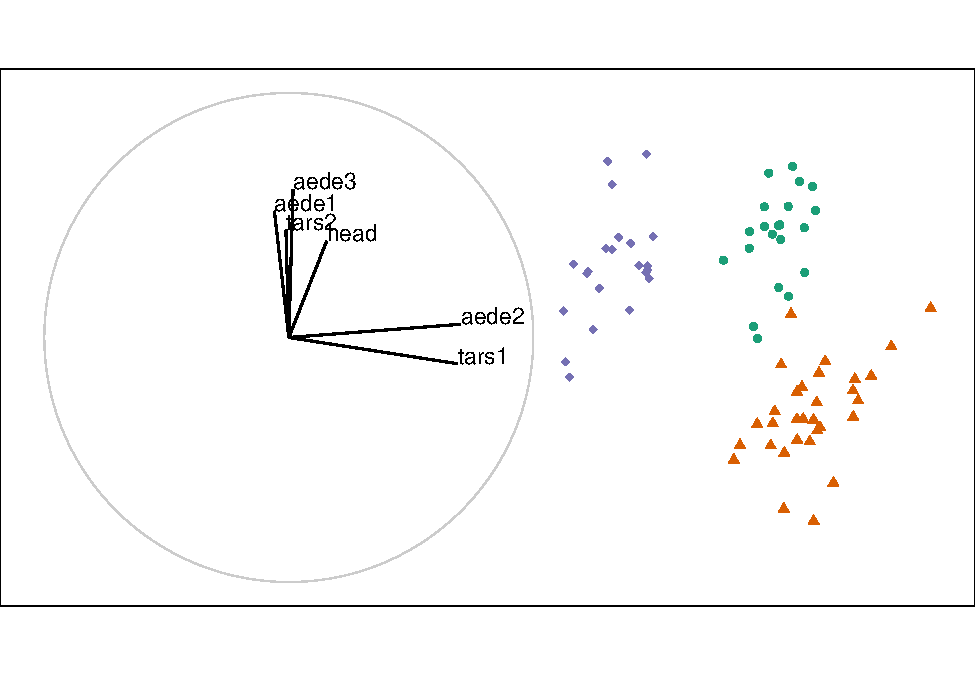
\includegraphics[width=0.7\linewidth]{spinifex_paper_files/figure-latex/step0-1} 

}

\caption[Initial 2D projection]{Initial 2D projection: representation of the basis  (left) and resulting data projection (right) of standardized flea data. The color and shape of data points are mapped to beetle species. The basis was identified using a projection pursuit guided tour, with the holes index. The contribution of the variables aede2 and tars1 approximately contrasts the other variables. The visible structure in the projection are the three clusters corresponding to the three species. Produced with the function \code{view\_basis()}.}\label{fig:step0}
\end{figure}
\end{Schunk}

\hypertarget{step-1-choose-manip-variable}{%
\subsubsection{Step 1) Choose manip
variable}\label{step-1-choose-manip-variable}}

In Figure \ref{fig:step0} the contribution of the variables tars1 and
aede2 mostly contrast the contribution of the other four variables.
These two variables combined contribute in the direction of the
projection where the purple cluster is separated from the other two
clusters. The variable aede2 is selected as the manip var, the variable
to be controlled in the tour. The question that will be explored, is,
how important this variable is to the separation of the clusters.

\hypertarget{step-2-create-the-3d-manip-space}{%
\subsubsection{Step 2) Create the 3D manip
space}\label{step-2-create-the-3d-manip-space}}

Initialize the coordinate basis vector as a zero vector \(\textbf{e}\)
of length \(p\), and set the \(k\)-th element to 1. In the example data,
aede2 is the fifth variable in the data, so \(k=5\), set \(e_5=1\). Use
a Gram-Schmidt process to orthonormalize the coordinate basis vector on
the original 2D projection to describe a 3D manip space, \(\textbf{M}\).

\begin{align*}
  e_k &\leftarrow 1 \\ 
  \textbf{e}^*_{[p,~1]} &= \textbf{e} - \langle \textbf{e}, \textbf{B}_1 \rangle \textbf{B}_1 - \langle \textbf{e}, \textbf{B}_2 \rangle \textbf{B}_2 \\ 
  \textbf{M}_{[p,~3]} &= (\textbf{B}_1,\textbf{B}_2,\textbf{e}^*)
\end{align*}

The manip space provides a 3D projection from \(p\)-dimensional space,
where the coefficient of the manip var can range completely between
{[}0, 1{]}. 3D rotation can be used to rotate the manip variable
completely into or completely out of a 2D projection. Figure
\ref{fig:step2} illustrates this 3D manip space with the manip var
highlighted. This representation is produced by calling the
\code{view\_manip\_space()} function. This diagram is purely used to
help explain the algorithm.

\begin{Schunk}
\begin{figure}

{\centering 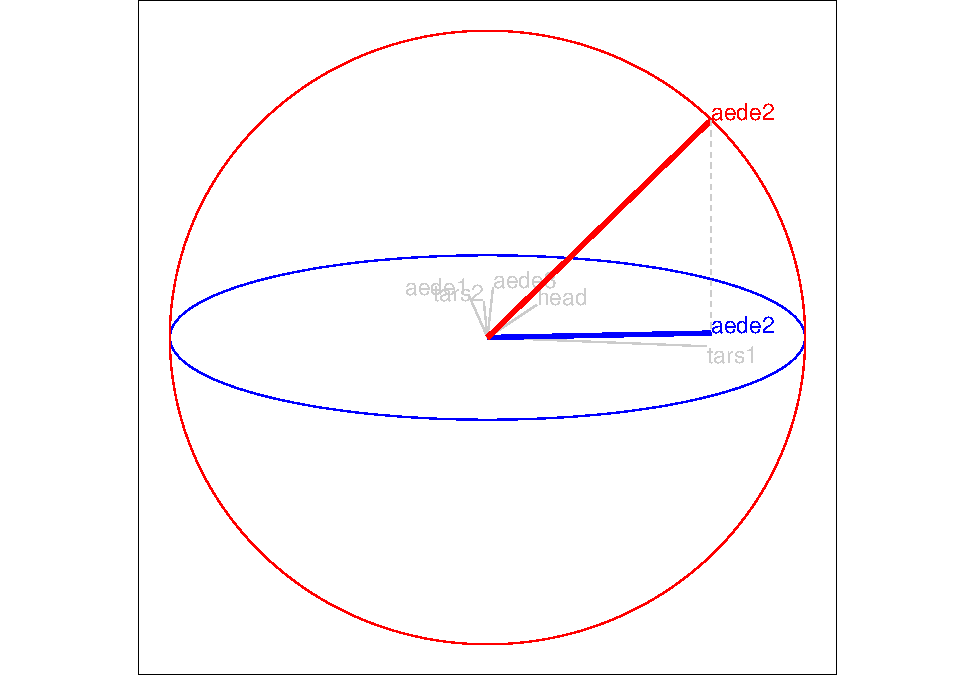
\includegraphics[width=0.7\linewidth]{spinifex_paper_files/figure-latex/step2-1} 

}

\caption[Illustration of a 3D manip space, constructed to change the contribution of the variable aede2 in the example data]{Illustration of a 3D manip space, constructed to change the contribution of the variable aede2 in the example data. The red circle indicates a unit sphere. The 2D projection is represented by the blue circle, with the projection coefficients represented by grey lines and text. The manip var axis, in red, has length 1 touching the sphere, extends the projection to a third dimension. The shadow of this axis (blue) is its contribution in the original 2D projection. Illustrated with the \code{view\_manip\_space()} function.}\label{fig:step2}
\end{figure}
\end{Schunk}

\hypertarget{step-3-defining-a-3d-rotation}{%
\subsubsection{Step 3) Defining a 3D
rotation}\label{step-3-defining-a-3d-rotation}}

The basis vector corresponding to the manip var (red line in Figure
\ref{fig:step2}), can be operated like a lever. This is the process of
the manual control, that rotates the manip variable into and out of the
2D projection (Figure \ref{fig:step3}). As the variable contribution is
controlled, the manip space rotates, and the projection onto the
horizontal projection plane correspondingly changes. This is a manual
tour. Generating a sequence of values for the rotation angles produces a
path for the rotation of the manip space.

For a radial tour, fix \(\theta\), the angle describing rotation within
the projection plane, and compute a sequence for \(\phi\), defining
movement out of the plane. This will change the initial value,
\(\phi_1\), the angle between \(\textbf{e}\) and its shadow in
\(\textbf{B}\), to a maximum of \(0\) (manip var fully in projection),
then to a minimum of \(\pi/2\) (manip var out of projection), before
returning to \(\phi_1\).

Rotations in 3D can be defined by the axes they pivot on. Rotation
within the projection, \(\theta\), is rotation around the \(Z\) axis.
Out-of-projection rotation, \(\phi\), is the rotation around an axis on
the \(XY\) plane, \(\textbf{U}\), orthogonal to \(\textbf{e}\). Given
these axes, the rotation matrix, \(\textbf{R}\) can be written as
follows, using Rodrigues' rotation formula (originally published in
Rodrigues (\protect\hyperlink{ref-rodrigues_lois_1840}{1840})):

\begin{align*}
    \textbf{R}_{[3,~3]} 
    &= \textbf{I}_3 + s_\phi\*\textbf{U} + (1-c_\phi)\*\textbf{U}^2 \\
        &=
    \begin{bmatrix}
      1 & 0 & 0 \\ 
      0 & 1 & 0 \\ 
      0 & 0 & 1 \\
    \end{bmatrix} +
    \begin{bmatrix}
      0 & 0 & c_\theta s_\phi \\
      0 & 0 & s_\theta s_\phi \\
      -c_\theta s_\phi & -s_\theta s_\phi & 0 \\
    \end{bmatrix} +
    \begin{bmatrix}
      -c_\theta (1-c_\phi) & s^2_\theta (1-c_\phi) & 0 \\
      -c_\theta s_\theta (1-c_\phi) & -s^2_\theta (1-c_\phi) & 0 \\
      0 & 0 & c_\phi-1 \\
    \end{bmatrix} \\
    &= 
    \begin{bmatrix}
      c_\theta^2 c_\phi + s_\theta^2 &
      -c_\theta s_\theta (1 - c_\phi) &
      -c_\theta s_\phi \\
      -c_\theta s_\theta (1 - c_\phi) &
      s_\theta^2 c_\phi + c_\theta^2 &
      -s_\theta s_\phi \\
      c_\theta s_\phi &
      s_\theta s_\phi &
      c_\phi
    \end{bmatrix} \\
\end{align*}

\noindent where

\begin{align*}
  \textbf{U} &= (u_x, u_y, u_z) =
  (s_\theta, -c_\theta, 0) \\ 
  &=
  \begin{bmatrix}
  0 & -u_z & u_y  \\
  u_z & 0 & -u_x \\
  -u_y & u_x & 0 \\
  \end{bmatrix} =
  \begin{bmatrix}
    0 & 0 & -c_\theta \\
    0 & 0 & -s_\theta \\
    c_\theta & s_\theta & 0 \\
  \end{bmatrix} \\
  \end{align*}

\hypertarget{step-4-creating-an-animation-of-the-radial-rotation}{%
\subsubsection{Step 4) Creating an animation of the radial
rotation}\label{step-4-creating-an-animation-of-the-radial-rotation}}

The steps outlined above can be used to create any arbitrary rotation in
the manip space. To use these for sensitivity analysis, the radial
rotation is built into an animation where the manip var is rotated fully
into the projection, completely out, and then back to the initial value.
This involves allowing \(\phi\) to vary between \(0\) and \(\pi/2\),
call the steps \(\phi_i\).

\begin{Schunk}
\begin{figure}

{\centering 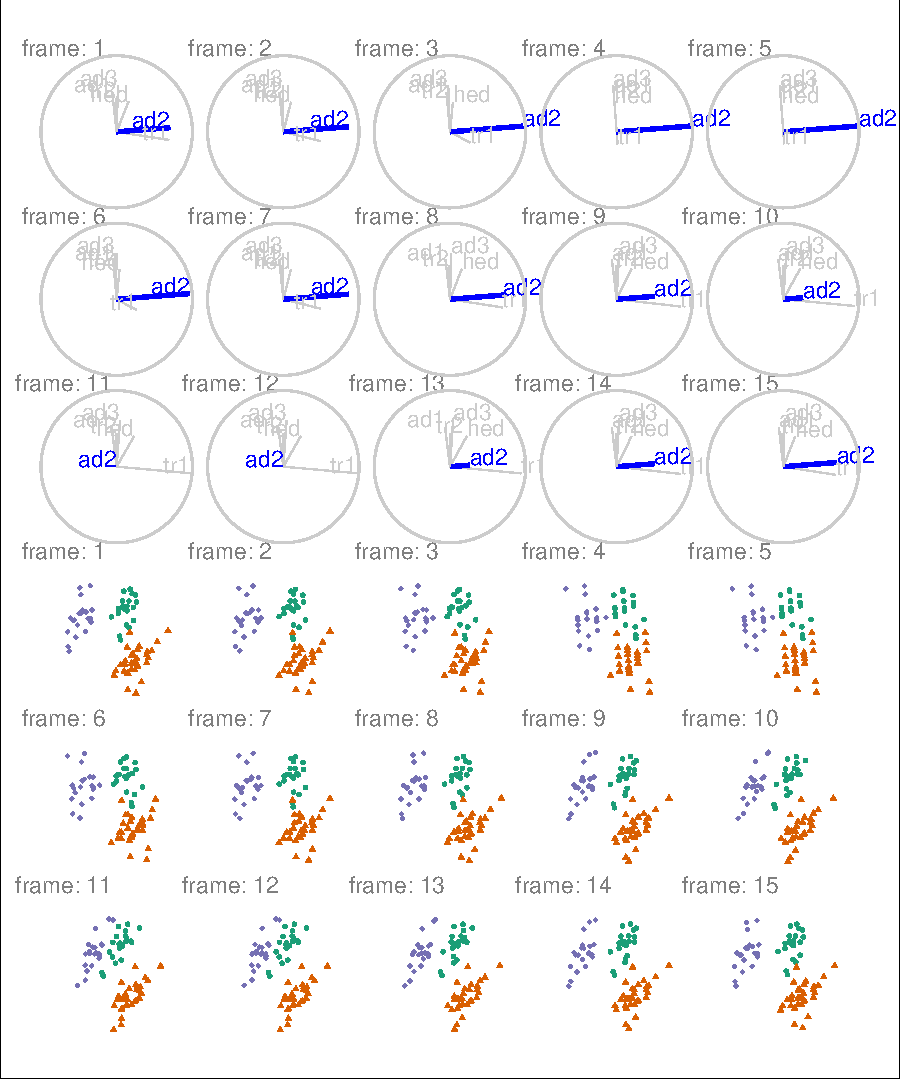
\includegraphics[width=1\linewidth]{spinifex_paper_files/figure-latex/step3-1} 

}

\caption[Snapshots of a radial manual tour manipulating aede2]{Snapshots of a radial manual tour manipulating aede2: (1) original projection, (2) full contribution, (3) zero contribution, (4) back to original. }\label{fig:step3}
\end{figure}
\end{Schunk}

\begin{enumerate}
\def\labelenumi{\arabic{enumi}.}
\tightlist
\item
  Set initial value of \(\phi_1\) and \(\theta\):
  \(\phi_1 = \cos^{-1}{\sqrt{B_{k1}^2+B_{k2}^2}}\),
  \(\theta = \tan^{-1}\frac{B_{k2}}{B_{k1}}\). \(\phi_1\) is the angle
  between \(\textbf{e}\) and its shadow in \(\textbf{B}\).
\item
  Set an angle increment (\(\Delta_\phi\)) that sets the step size for
  the animation, to rotate the manip var into and out of the projection.
  (Note: Using angle increment, rather than a number of steps, to
  control the movement, is consistent with the tour algorithm as
  implemented in the \pkg{tourr}).
\item
  Step towards \(0\), where the manip var is completely in the
  projection.
\item
  Step towards \(\pi/2\), where the manip variable has no contribution.
\item
  Step back to \(\phi_1\).
\end{enumerate}

In each of the steps 3-5, a small step may be added to ensure that the
endpoints of \(\phi\) (\(0\), \(\pi/2\)) are reached.

\hypertarget{sec:display}{%
\subsubsection{Step 5) Projecting the data}\label{sec:display}}

The operation of a manual tour is defined on the projection bases. Only
when the data plot needs to be made is the data projected into the
relevant basis.

\begin{align*}
  \textbf{Y}^{(i)}_{[n,~3]} &= \textbf{X}_{[n,~p]} \textbf{M}_{[p,~3]} \textbf{R}^{(i)}_{[3,3]}
\end{align*}

\noindent where \(\textbf{R}^{(i)}_{[3,3]}\) is the incremental rotation
matrix, using \(\phi_i\). To make the data plot, use the first two
columns of \textbf{Y}. Show the projected data for each frame in
sequence to form an animation.

Figure \ref{fig:step4} illustrates a manual tour sequence having 15
steps. The projection axes are displayed on the top half, which
corresponds to the projected data in the bottom half. When aede2 is
removed from the projection, the purple cluster overlaps with the green
cluster. This suggests that aede2 is important for distinguishing this
species.

Tours are typically viewed as an animation. The animation of this tour
can be viewed online at
\url{https://nspyrison.netlify.com/thesis/flea_manualtour_mvar5/}. The
page may take a moment to load. Animations can be produced using the
function \code{play\_manual\_tour()}.

\begin{Schunk}
\begin{figure}

{\centering 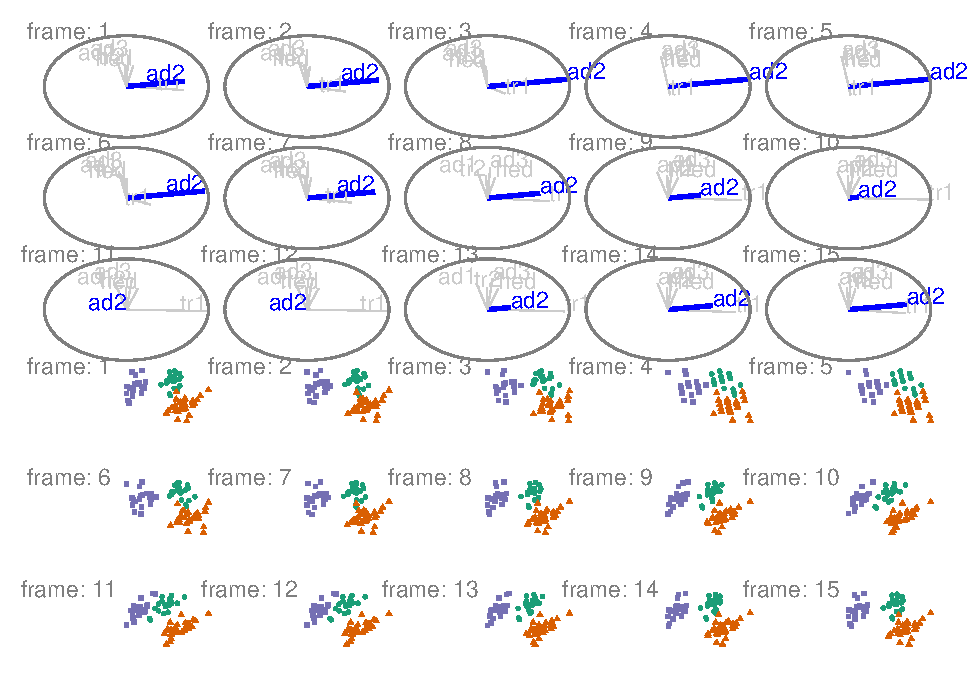
\includegraphics[width=5.83in,height=7in]{spinifex_paper_files/figure-latex/step4-1} 

}

\caption[Radial manual tour manipulating aede2 of standardized flea data]{Radial manual tour manipulating aede2 of standardized flea data. The axis for aede2 increases in contribution to the projection, from its initial value to 1, decreasing to 0 and then returning to the initial value. This affects the separatiion between the purple and green clusters. This shows that aede2 is important for distinguishing the purple species, because the separation disappears when aede2 is not contributing to the projection. An animation can be viewed at https://nspyrison.netlify.com/thesis/flea\_manualtour\_mvar5/.}\label{fig:step4}
\end{figure}
\end{Schunk}

\hypertarget{sec:usage}{%
\section{Package structure and functionality}\label{sec:usage}}

This section describes the functions available in the package, and how
to use them.

\hypertarget{installation}{%
\subsection{Installation}\label{installation}}

The \pkg{spinifex} is available from CRAN, and can be installed by:

\begin{Schunk}
\begin{Sinput}
install.package("spinifex")
library("spinifex")
\end{Sinput}
\end{Schunk}

\noindent Also see the vignette for examples of usage:

\begin{verbatim}
vignette("spinifex_vignette")
\end{verbatim}

\noindent The development version can be installed from github:

\begin{verbatim}
remotes::install_github("nspyrison/spinifex") 
\end{verbatim}

\hypertarget{functions}{%
\subsection{Functions}\label{functions}}

Table \ref{tab:functionsTable} lists the primary functions and their
purpose. These are grouped into four types: construction for building a
tour path, render to make the plot objects, animation for running the
animation, and specialty for providing illustrations used in the
algorithm description.

\begin{Schunk}
\begin{table}[t]

\caption{\label{tab:functionsTable}Summary of available functions.}
\centering
\begin{tabular}{lll}
\toprule
Type & Function & Description\\
\midrule
construction & create\_manip\_space & forms the 3D space of rotation\\
construction & rotate\_manip\_space & performs 3D rotation\\
construction & manual\_tour & generates sequence of 2D frames\\
 &  & \\
render & render\_ & constructs the ggplot object to feed to animation\\
render & render\_plotly & converts the ggplot object to a plotly animation\\
render & render\_gganimate & converts the ggplot object to a gganimate  animation\\
render & array2df & turns a tour path array into long form, for plotting\\
 &  & \\
animation & play\_tour\_path & animates given tour path\\
animation & play\_manual\_tour & animates the manual tour algorithm\\
 &  & \\
specialty & view\_basis & displays the reference frame of a given basis\\
specialty & view\_manip\_space & illustrative display of any manip space\\
\bottomrule
\end{tabular}
\end{table}

\end{Schunk}

\hypertarget{usage}{%
\subsection{Usage}\label{usage}}

Using the \code{flea} data from the \pkg{tourr} package, we will
illustrate generating a manual tour to explore the sensitivity of the
cluster structure is to the variable aede2.

\begin{Schunk}
\begin{Sinput}
library(spinifex)
f_data  <- tourr::rescale(flea[, 1:6])                    ## standardize data
f_path  <- save_history(f_data, guided_tour(holes()))     ## guided tour using holes index
f_basis <- matrix(f_path[,, max(dim(f_path)[3])], ncol=2) ## optimal projection
f_cat   <- factor(flea$species)                           ## categorical var
f_mvar  <- 5                                              ## set manip var
angle_speed <- .26
play_manual_tour(data = f_data,                           ## Generates animation
                 basis = f_basis,                         ## using plotly
                 manip_var = f_mvar, 
                 angle = angle_speed,
                 col = f_cat,
                 pch = f_cat)
\end{Sinput}
\end{Schunk}

The \code{play\_manual\_tour()} function is a composite function for
user convenience that does these operations:

\begin{Schunk}
\begin{Sinput}
manual_tour()
array2df()
render_plotly()
\end{Sinput}
\end{Schunk}

\noindent This will generate an html animation using plotly. Switching
the renderer to \code{gganimate} is an option, which will also create an
html animation or an animated gif. Each of these formats allows for the
animation to be made available on a web site, or directly visible in an
html formatted document.

\hypertarget{making-illustrations}{%
\subsubsection{Making illustrations}\label{making-illustrations}}

The function \texttt{view\_basis} can be used to show a projection, just
the basis, or with the data overlaid. For example, the plots in Figures
\ref{fig:step0} and \ref{fig:step3} were made with code similar to this:

\begin{Schunk}
\begin{Sinput}
view_basis(basis = f_basis, 
           data = f_data,
           labels = colnames(f_data))
\end{Sinput}
\end{Schunk}

\noindent An illustration of the manip space (as shown in Figure
\ref{fig:step2}) is made with the \texttt{view\_manip\_space} function,
as follows:

\begin{Schunk}
\begin{Sinput}

view_manip_space(basis = f_basis, 
                 manip_var = f_mvar, 
                 labels = colnames(f_data))
\end{Sinput}
\end{Schunk}

\hypertarget{sec:application}{%
\section{Application}\label{sec:application}}

Wang et al. (\protect\hyperlink{ref-wang_mapping_2018}{2018}) introduce
a new tool, PDFSense, to visualize the sensitivity of hadronic
experiments to nucleon structure. The parameter-space of these
experiments lies in 56 dimensions, \(\delta \in \mathbb{R}^{56}\), and
are visualized as 3D subspaces of the 10 first principal components in
linear (PCA) and non-linear (t-SNE) embeddings.

Cook, Laa, and Valencia
(\protect\hyperlink{ref-cook_dynamical_2018}{2018}) illustrates how to
learn more about the structures using a grand tour. Tours are able to
better resolve the shape of clusters, intra-cluster detail, and better
outlier detection than PDFSense \& TFEP (TensorFlow embedded
projections) or traditional static embeddings. This example builds from
here, illustrating how the manual tour can be used to examine the
sensitivity of structure in a projection to different parameters. The
specific 2D projections passed to the manual tour were provided from
Cook, Laa, and Valencia
(\protect\hyperlink{ref-cook_dynamical_2018}{2018}).

The data has a hierarchical structure with top-level clusters; DIS, VBP,
and jet. Each cluster is a particular class of experiments, each with
many experimental datasets which, in turn, have many observations. In
consideration of data density, we conduct manual tours on subsets of the
DIS and jet clusters. This explores the sensitivity of the structure to
each of the variables in turn and we present the subjectively best and
worst variable to manipulate for identifying dimensionality of the
clusters and describing the span of the clusters.

\hypertarget{jet-cluster}{%
\subsection{Jet cluster}\label{jet-cluster}}

The jet cluster resides in a smaller dimensionality than the full set of
experiments with four principal components explaining 95\% of the
variation in the cluster (Cook, Laa, and Valencia
\protect\hyperlink{ref-cook_dynamical_2018}{2018}). The data within this
4D embedding is further subsetted, to ATLAS7old and ATLAS7new, in order
to focus on two groups, with a reasonable number of observations, that
occupy different parts of the subspace. Radial manual tours controlling
contributions from PC4 and PC3 are shown in Figures
\ref{fig:JetClusterGood} and \ref{fig:JetClusterBad}, respectively. The
difference in shape can be interpreted as the experiments probing
different phase-spaces. Back-transforming the principal components to
the original variables can be done for more detailed interpretation.

When PC4 is removed from the projection (Figure
\ref{fig:JetClusterGood}), the difference between the two groups is
removed, indicating that it is important for distinguishing experiments.
However, removing PC3 from the projection (Figure
\ref{fig:JetClusterBad}), has no effect on the structure, indicating it
is not important for distinguishing experiments.

Animations for the remaining PCs can be viewed at the following links:
\href{https://nspyrison.netlify.com/thesis/jetcluster_manualtour_pc1/}{PC1},
\href{https://nspyrison.netlify.com/thesis/jetcluster_manualtour_pc2/}{PC2},
\href{https://nspyrison.netlify.com/thesis/jetcluster_manualtour_pc3/}{PC3},
and
\href{https://nspyrison.netlify.com/thesis/jetcluster_manualtour_pc4/}{PC4}.
It can be seen that only PC4 is important for viewing the difference in
these two experiments.

\begin{Schunk}
\begin{figure}

{\centering 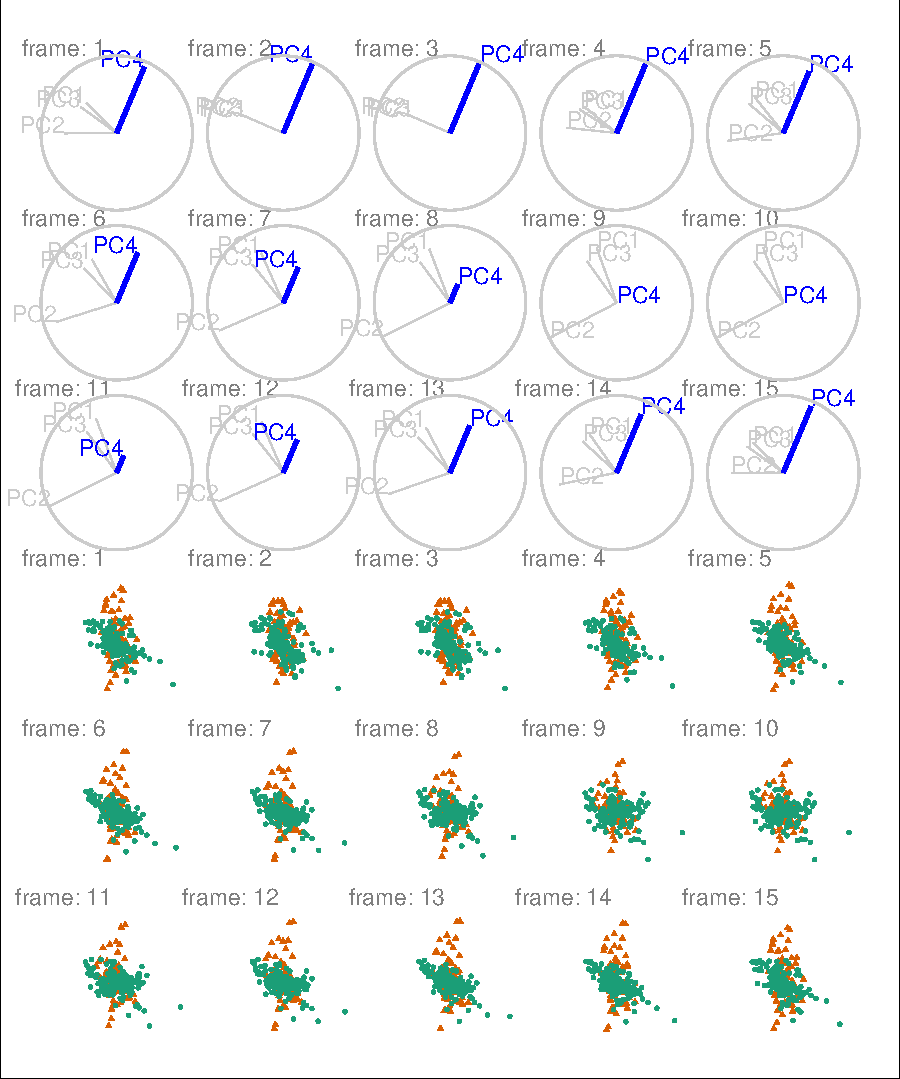
\includegraphics[width=5.83in,height=7in]{spinifex_paper_files/figure-latex/JetClusterGood-1} 

}

\caption[Snapshots of a radial manual tour of PC4 focusing on the jet cluster, with color indicating experiment type]{Snapshots of a radial manual tour of PC4 focusing on the jet cluster, with color indicating experiment type: ATLAS7new (green) and ATLAS7old (orange).  When PC4 is removed from the projection (frame 10) there is little difference between the groups, suggesting that PC4 is important for distinguishing the experiments.  The animation can be viewed at https://nspyrison.netlify.com/thesis/jetcluster\_manualtour\_pc4/.}\label{fig:JetClusterGood}
\end{figure}
\end{Schunk}

\begin{Schunk}
\begin{figure}

{\centering 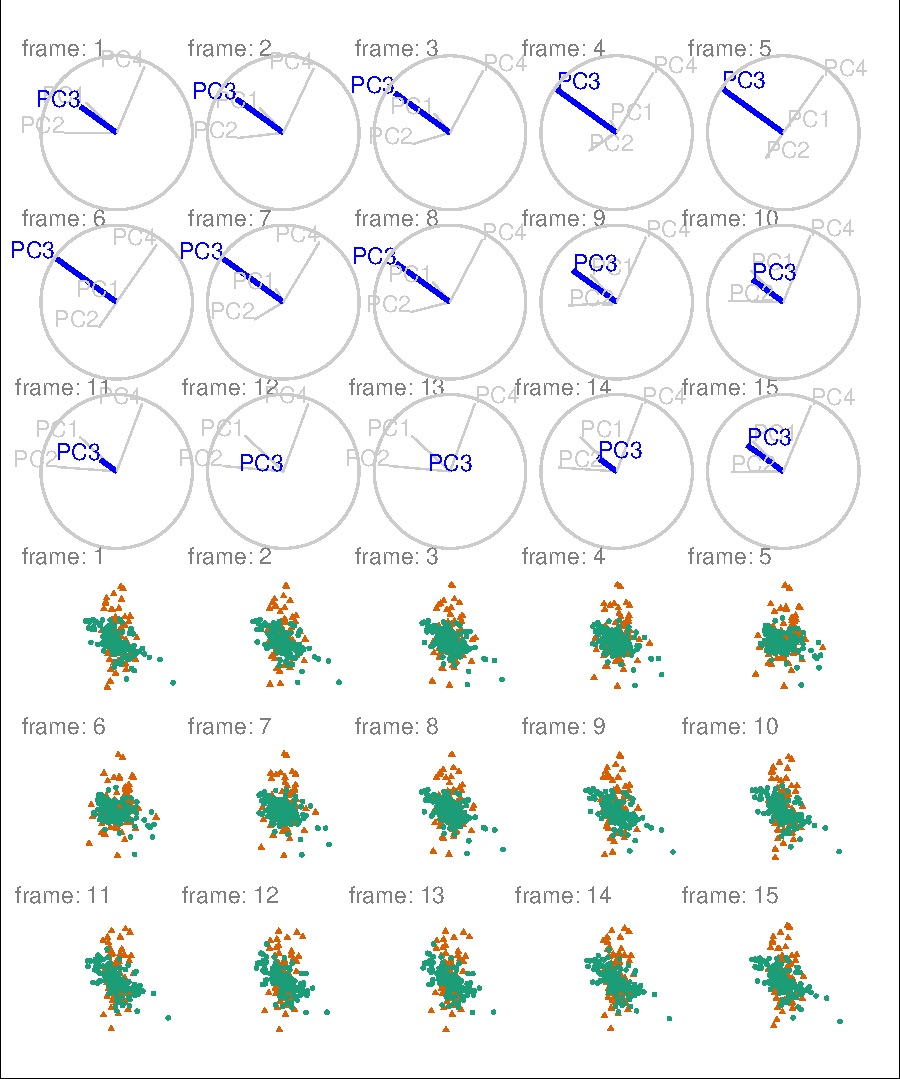
\includegraphics[width=5.83in,height=7in]{spinifex_paper_files/figure-latex/JetClusterBad-1} 

}

\caption[Snapshots of a radial manual tour of PC3 focusing on the jet cluster, with color indicating experiment type]{Snapshots of a radial manual tour of PC3 focusing on the jet cluster, with color indicating experiment type: ATLAS7new (green) and ATLAS7old (orange).  When the contribution of PC3 is changed there is little change to the structure of the two groups, suggesting that PC3 is not important for distinguishing the experiments. The animation can be viewed at https://nspyrison.netlify.com/thesis/jetcluster\_manualtour\_pc3/.}\label{fig:JetClusterBad}
\end{figure}
\end{Schunk}

\hypertarget{dis-cluster}{%
\subsection{DIS cluster}\label{dis-cluster}}

Following Cook, Laa, and Valencia
(\protect\hyperlink{ref-cook_dynamical_2018}{2018}), to explore the DIS
cluster, PCA is recomputed and the first six principal components,
explaining 48\% of the variation is used. The contributions of PC6 and
PC2 are explored in Figures \ref{fig:DISclusterGood} and
\ref{fig:DISclusterBad}, respectively. Three experiments are examined:
DIS HERA1+2 (green), dimuon SIDIS (purple), and charm SIDIS (orange).

Both PC2 and PC6 contribute to the projection similarly. When PC6 is
rotated into the projection, variation in the DIS HERA1+2 is greatly
reduced. When PC2 is removed from the projection, dimuon SIDIS becomes
more clearly distinct. Even though both variables contribute similarly
to the original projection, their contributions have quite different
effects on the structure of each cluster, and the distinction between
clusters. Animations of all of the principal components can be viewed
from the links:
\href{https://nspyrison.netlify.com/thesis/discluster_manualtour_pc1/}{PC1},
\href{https://nspyrison.netlify.com/thesis/discluster_manualtour_pc2/}{PC2},
\href{https://nspyrison.netlify.com/thesis/discluster_manualtour_pc3/}{PC3},
\href{https://nspyrison.netlify.com/thesis/discluster_manualtour_pc4/}{PC4},
\href{https://nspyrison.netlify.com/thesis/discluster_manualtour_pc5/}{PC5},
and
\href{https://nspyrison.netlify.com/thesis/discluster_manualtour_pc6/}{PC6}.

\begin{Schunk}
\begin{figure}

{\centering 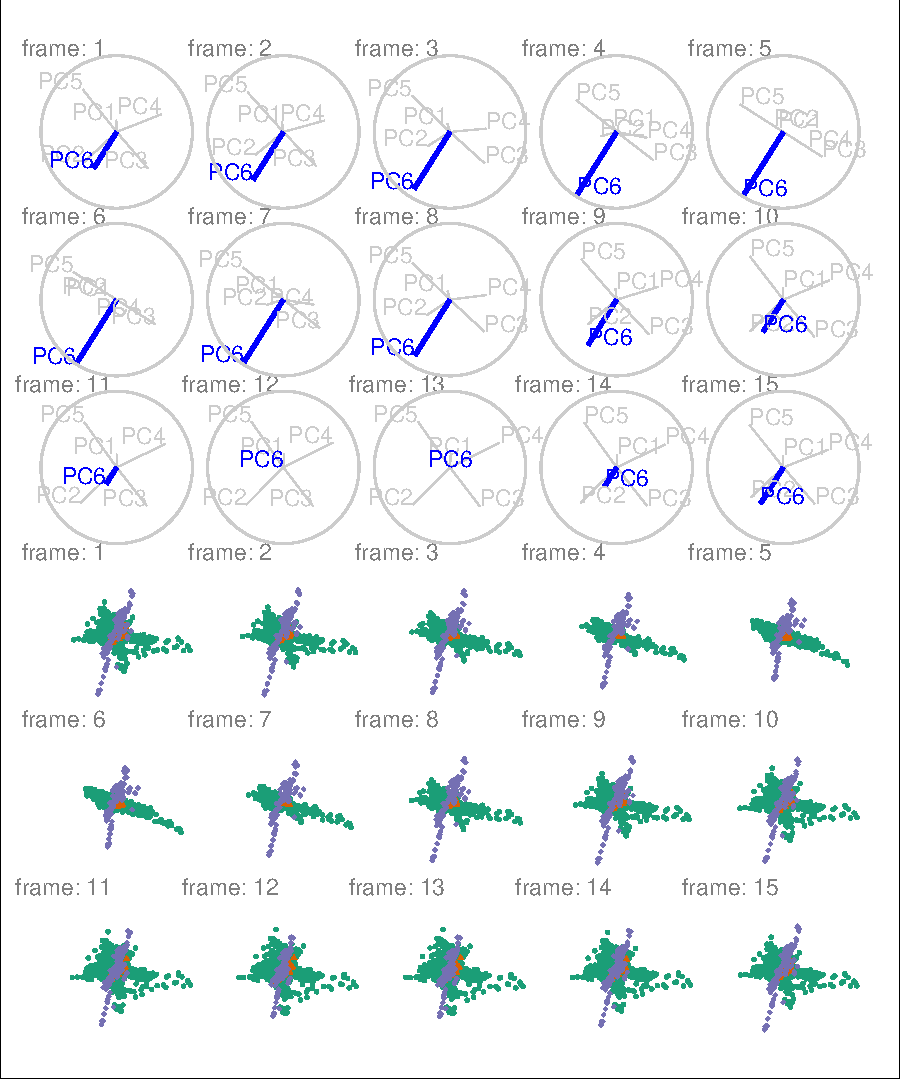
\includegraphics[width=5.83in,height=7in]{spinifex_paper_files/figure-latex/DISclusterGood-1} 

}

\caption[Snapshots of a radial manual tour exploring the contribution of PC6 for the DIS cluster, with color indicating experiment type]{Snapshots of a radial manual tour exploring the contribution of PC6 for the DIS cluster, with color indicating experiment type: DIS HERA1+2 (green), dimuon SIDIS (purple), and charm SIDIS (orange). DIS HERA1+2 is distributed in a cross-shaped plane, charm SIDIS occupies the center of this cross, and dimuon SIDIS is a linear cluster crossing DIS HERA1+2. As PC6's contribution is increased, DIS HERA1+2 becomes almost singular in one direction (frame 5), indicating that this experiment has very little variability in the direction of PC6.  The animation can be viewed at https://nspyrison.netlify.com/thesis/discluster\_manualtour\_pc6/.}\label{fig:DISclusterGood}
\end{figure}
\end{Schunk}

\begin{Schunk}
\begin{figure}

{\centering 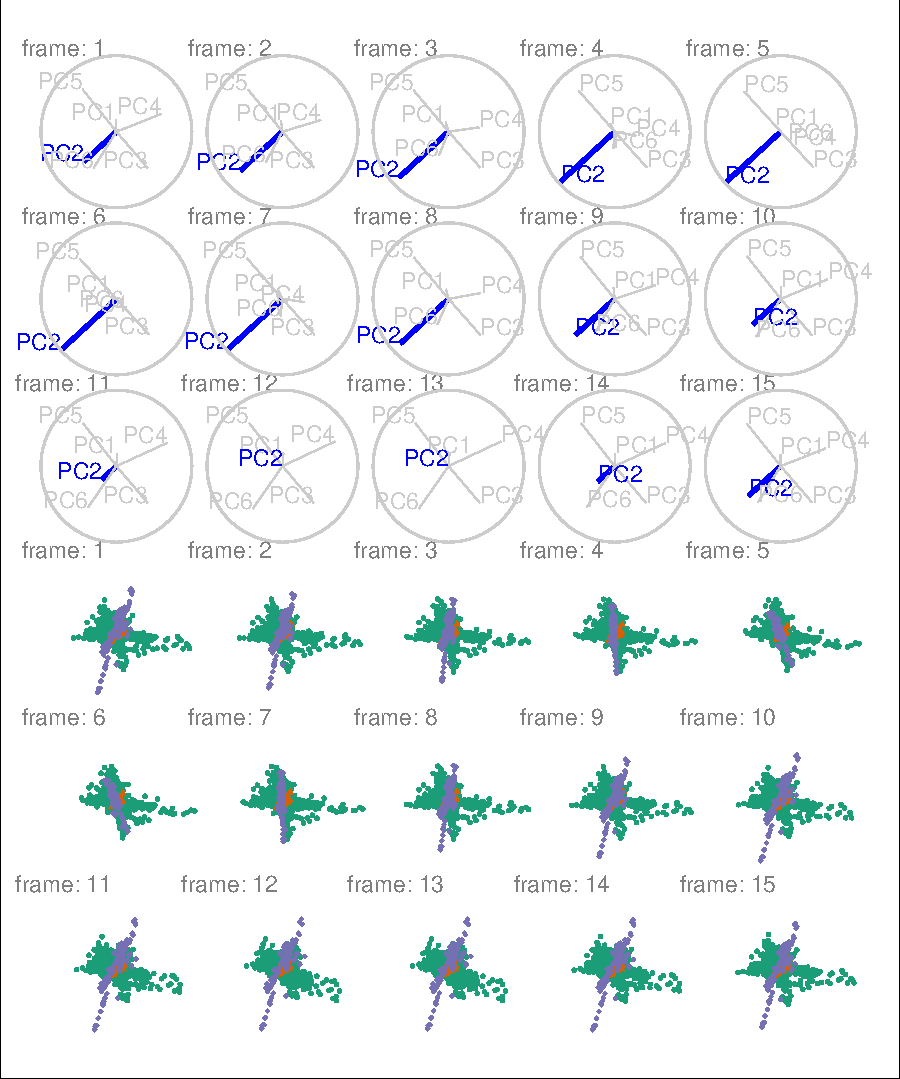
\includegraphics[width=5.83in,height=7in]{spinifex_paper_files/figure-latex/DISclusterBad-1} 

}

\caption[Snapshots of a radial manual tour exploring the contribution of PC2 for the DIS cluster, with color indicating experiment type]{Snapshots of a radial manual tour exploring the contribution of PC2 for the DIS cluster, with color indicating experiment type: DIS HERA1+2 (green), dimuon SIDIS (purple), and charm SIDIS (orange). As PC2's contribution is decreased, dimuon SIDIS becomes more distinguishable from the other two clusters (frames 10-14), indicating that in its absence PC2 is important.  The animation can be viewed at https://nspyrison.netlify.com/thesis/discluster\_manualtour\_pc2/.}\label{fig:DISclusterBad}
\end{figure}
\end{Schunk}

\hypertarget{sec:discussion}{%
\section{Discussion}\label{sec:discussion}}

Dynamic linear projections of numeric multivariate data, tours, play an
important role in data visualization; they extend the dimensionality of
visuals to peek into high-dimensional data and parameter spaces. This
research has taken the manual tour algorithm, specifically the radial
rotation, used in GGobi (Swayne et al.
\protect\hyperlink{ref-swayne_ggobi:_2003}{2003}) to interactively
rotate a variable into or out of a 2D projection, and modified it to
create an animation that performs the same task. It is most useful for
examining the importance of variables, and how the structure in the
projection is sensitive or not to specific variables. This functionality
available in package \pkg{spinifex}. The work complements the methods
available in the \pkg{tourr} package.

This work was motivated by problems in physics, and thus the usage was
illustrated on data comparing experiments of hadronic collisions, to
explore the sensitivity of cluster structure to different principal
components. These tools can be applied quite broadly, to many
multivariate data analysis problems.

The manual tour is constrained in the sense that the effect of one
variable is dependent on the contributions of other variables in the
manip space. However, this can be useful to simplify a projection, to
remove variables without affecting the visible structure. Defining a
manual rotation in high dimensions is possible using Givens rotations
and Householder reflections as outlined in Buja et al.
(\protect\hyperlink{ref-buja_computational_2005}{2005}). This would
provide more flexible manual rotation, but more difficult for a user
because they have the choice (too much choice) of which directions to
move.

Another future research topic could be to extend the algorithm for use
on 3D projections. With the current popularity and availability of 3D
virtual displays, this may benefit the detection and understanding of
the higher dimensional structure, or enable the examination of
functions.

Having a graphical user interface would be useful for making it easier
and more accessible to a general audience. This is possible to implement
using \CRANpkg{shiny} (Chang et al.
\protect\hyperlink{ref-chang_shiny:_2018}{2018}). The primary purposes
of the interface would be to allow the user to interactively change the
manip variable easily, and the interpolation step for more or less
detailed views.

\hypertarget{acknowledgments}{%
\section{Acknowledgments}\label{acknowledgments}}

This article was created in R (R Core Team
\protect\hyperlink{ref-r_core_team_r:_2019}{2019}), using
\CRANpkg{knitr} (Xie \protect\hyperlink{ref-stodden_knitr:_2014}{2014})
and \CRANpkg{rmarkdown} (Xie, Allaire, and Grolemund
\protect\hyperlink{ref-xie_r_2018}{2018}), with code generating the
examples inline. The source files for this article be found at
\href{https://github.com/nspyrison/spinifex_paper/}{github.com/nspyrison/spinifex\_paper/}.
The source code for the \pkg{spinifex} package can be found at
\href{https://github.com/nspyrison/spinifex/}{github.com/nspyrison/spinifex/}.

\hypertarget{bibliography}{%
\section*{Bibliography}\label{bibliography}}
\addcontentsline{toc}{section}{Bibliography}

\hypertarget{refs}{}
\leavevmode\hypertarget{ref-asimov_grand_1985}{}%
Asimov, Daniel. 1985. ``The Grand Tour: A Tool for Viewing
Multidimensional Data.'' \emph{SIAM Journal on Scientific and
Statistical Computing} 6 (1): 128--43.
\url{https://doi.org/https://doi.org/10.1137/0906011}.

\leavevmode\hypertarget{ref-buja_computational_2005}{}%
Buja, Andreas, Dianne Cook, Daniel Asimov, and Catherine Hurley. 2005.
``Computational Methods for High-Dimensional Rotations in Data
Visualization.'' In \emph{Handbook of Statistics}, 24:391--413.
Elsevier. \url{https://doi.org/10.1016/S0169-7161(04)24014-7}.

\leavevmode\hypertarget{ref-chang_shiny:_2018}{}%
Chang, Winston, Joe Cheng, J. J. Allaire, Yihui Xie, and Jonathan
McPherson. 2018. \emph{Shiny: Web Application Framework for R}.
\url{https://CRAN.R-project.org/package=shiny}.

\leavevmode\hypertarget{ref-cook_manual_1997}{}%
Cook, Dianne, and Andreas Buja. 1997. ``Manual Controls for
High-Dimensional Data Projections.'' \emph{Journal of Computational and
Graphical Statistics} 6 (4): 464--80.
\url{https://doi.org/10.2307/1390747}.

\leavevmode\hypertarget{ref-cook_grand_1995}{}%
Cook, Dianne, Andreas Buja, Javier Cabrera, and Catherine Hurley. 1995.
``Grand Tour and Projection Pursuit.'' \emph{Journal of Computational
and Graphical Statistics} 4 (3): 155.
\url{https://doi.org/10.2307/1390844}.

\leavevmode\hypertarget{ref-cook_dynamical_2018}{}%
Cook, Dianne, Ursula Laa, and German Valencia. 2018. ``Dynamical
Projections for the Visualization of PDFSense Data.'' \emph{Eur. Phys.
J. C} 78 (9): 742. \url{https://doi.org/10.1140/epjc/s10052-018-6205-2}.

\leavevmode\hypertarget{ref-kirkpatrick_optimization_1983}{}%
Kirkpatrick, Scott, C. Daniel Gelatt, and Mario P. Vecchi. 1983.
``Optimization by Simulated Annealing.'' \emph{Science} 220 (4598):
671--80. \url{https://doi.org/10.1126/science.220.4598.671}.

\leavevmode\hypertarget{ref-lubischew_use_1962}{}%
Lubischew, Alexander A. 1962. ``On the Use of Discriminant Functions in
Taxonomy.'' \emph{Biometrics}, 455--77.
\url{https://doi.org/10.2307/2527894}.

\leavevmode\hypertarget{ref-pedersen_gganimate:_2019}{}%
Pedersen, Thomas Lin, and David Robinson. 2019. \emph{Gganimate: A
Grammar of Animated Graphics}.
\url{http://github.com/thomasp85/gganimate}.

\leavevmode\hypertarget{ref-r_core_team_r:_2019}{}%
R Core Team. 2019. \emph{R: A Language and Environment for Statistical
Computing}. Vienna, Austria: R Foundation for Statistical Computing.
\url{https://www.R-project.org/}.

\leavevmode\hypertarget{ref-rodrigues_lois_1840}{}%
Rodrigues, Olinde. 1840. \emph{Des Lois Géométriques Qui Régissent Les
Déplacements d'un Système Solide Dans L'espace: Et de La Variation Des
Cordonnées Provenant de Ces Déplacements Considérés Indépendamment Des
Causes Qui Peuvent Les Produire}.

\leavevmode\hypertarget{ref-sievert_plotly_2018}{}%
Sievert, Carson. 2018. \emph{Plotly for R}.
\url{https://plotly-book.cpsievert.me}.

\leavevmode\hypertarget{ref-swayne_ggobi:_2003}{}%
Swayne, Deborah F, Duncan Temple Lang, Andreas Buja, and Dianne Cook.
2003. ``GGobi: Evolving from XGobi into an Extensible Framework for
Interactive Data Visualization.'' \emph{Computational Statistics \& Data
Analysis}, Data Visualization, 43 (4): 423--44.
\url{https://doi.org/10.1016/S0167-9473(02)00286-4}.

\leavevmode\hypertarget{ref-wang_mapping_2018}{}%
Wang, Bo-Ting, T. J. Hobbs, Sean Doyle, Jun Gao, Tie-Jiun Hou, Pavel M.
Nadolsky, and Fredrick I. Olness. 2018. ``Mapping the Sensitivity of
Hadronic Experiments to Nucleon Structure.'' \emph{Physical Review D} 98
(9): 094030. \url{https://doi.org/10.1103/PhysRevD.98.094030}.

\leavevmode\hypertarget{ref-wickham_ggplot2:_2016}{}%
Wickham, Hadley. 2016. \emph{Ggplot2: Elegant Graphics for Data
Analysis}. Springer-Verlag New York. \url{http://ggplot2.org}.

\leavevmode\hypertarget{ref-wickham_tourr_2011}{}%
Wickham, Hadley, Dianne Cook, Heike Hofmann, and Andreas Buja. 2011.
``\textbf{Tourr} : An \emph{R} Package for Exploring Multivariate Data
with Projections.'' \emph{Journal of Statistical Software} 40 (2).
\url{https://doi.org/10.18637/jss.v040.i02}.

\leavevmode\hypertarget{ref-stodden_knitr:_2014}{}%
Xie, Yihui. 2014. ``Knitr: A Comprehensive Tool for Reproducible
Research in R.'' In \emph{Implementing Reproducible Computational
Research}, edited by Victoria Stodden, Friedrich Leisch, and Roger D.
Peng. Chapman; Hall/CRC.
\url{http://www.crcpress.com/product/isbn/9781466561595}.

\leavevmode\hypertarget{ref-xie_r_2018}{}%
Xie, Yihui, J. J. Allaire, and Garrett Grolemund. 2018. \emph{R
Markdown: The Definitive Guide}. Boca Raton, Florida: Chapman; Hall/CRC.
\url{https://bookdown.org/yihui/rmarkdown}.

\bibliography{spinifex\_paper.bib}

\address{%
Nicholas Spyrison\\
Monash University\\
Faculty of Information Technology\\
}
\href{mailto:nicholas.spyrison@monash.edu}{\nolinkurl{nicholas.spyrison@monash.edu}}

\address{%
Dianne Cook\\
Monash University\\
Department of Econometrics and Business Statistics\\
}
\href{mailto:dicook@monash.edu}{\nolinkurl{dicook@monash.edu}}

